\section{Xây dựng generic audit trigger function (PL/pgSQL)}

Hàm trigger tổng quát \texttt{func\_audit\_trigger()} là thành phần trung tâm của toàn bộ hệ thống \cite{PG16Triggers}. Nó được thiết kế để có thể gắn vào \textbf{bất kỳ bảng nghiệp vụ nào} mà không cần viết lại logic:

\begin{center}
\captionof{listing}{Hàm trigger Audit Log chung (PL/pgSQL)}
\label{lst:audit-trigger}
\begin{Verbatim}[frame=single, fontsize=\footnotesize, numbers=left, numbersep=5pt, breaklines]
CREATE OR REPLACE FUNCTION func_audit_trigger()
RETURNS TRIGGER AS $$
DECLARE
    v_table TEXT := TG_TABLE_SCHEMA || '.' || TG_TABLE_NAME;
BEGIN
    -- session_user = the actual connecting user
    -- (not affected by SECURITY DEFINER -- always equals app_user)
    IF (TG_OP = 'DELETE') THEN
        INSERT INTO audit_logs (table_name, operation, user_name, old_data)
        VALUES (v_table, 'DELETE', session_user, to_jsonb(OLD));
        RETURN OLD;
    ELSIF (TG_OP = 'UPDATE') THEN
        INSERT INTO audit_logs (table_name, operation, user_name, old_data, new_data)
        VALUES (v_table, 'UPDATE', session_user, to_jsonb(OLD), to_jsonb(NEW));
        RETURN NEW;
    ELSIF (TG_OP = 'INSERT') THEN
        INSERT INTO audit_logs (table_name, operation, user_name, new_data)
        VALUES (v_table, 'INSERT', session_user, to_jsonb(NEW));
        RETURN NEW;
    END IF;
    RETURN NULL;
END;
$$ LANGUAGE plpgsql
   SECURITY DEFINER
   SET search_path = public, pg_temp;
\end{Verbatim}
\end{center}

\textbf{Luồng xử lý:} \texttt{app\_user} thực hiện DML (\texttt{INSERT/UPDATE/DELETE}) trên các bảng nghiệp vụ $\rightarrow$ AFTER ROW trigger gọi \texttt{func\_audit\_trigger()} $\rightarrow$ ghi vào \texttt{audit\_logs} (partitioned) với dữ liệu \texttt{old\_data/new\_data} dạng JSONB trong cùng transaction.

\begin{center}
\centering
\makebox[\textwidth][c]{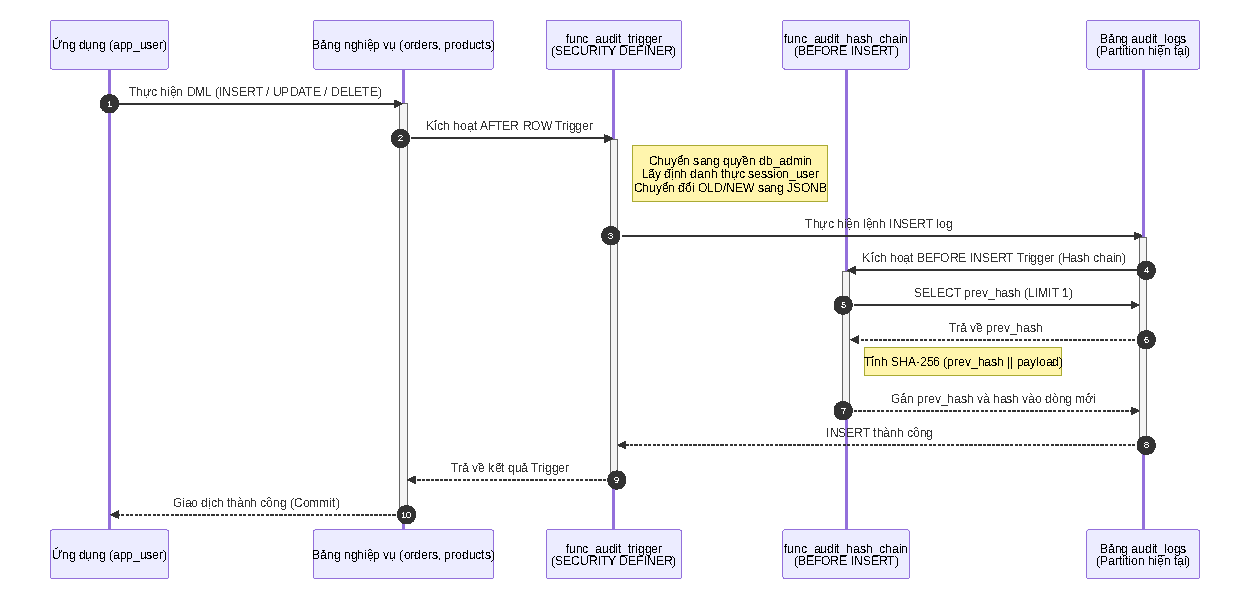
\includegraphics[width=\textwidth,height=0.85\textheight,keepaspectratio]{img/mermaid/seq_audit_write.pdf}}
\captionof{figure}{Sơ đồ tuần tự: Luồng ghi Audit Log qua Trigger}
\label{fig:seq-audit-write}
\end{center}

\section{Tự động hóa triển khai audit cho nhiều bảng (Dynamic Triggers)}

Hệ thống sử dụng một hàm trigger duy nhất có thể gắn vào bất kỳ bảng nghiệp vụ nào:

\begin{center}
\captionof{listing}{Tạo trigger cho bảng nghiệp vụ}
\label{lst:create-trigger}
\begin{Verbatim}[frame=single, fontsize=\footnotesize, numbers=left, numbersep=5pt, breaklines]
CREATE TRIGGER trg_audit_orders
AFTER INSERT OR UPDATE OR DELETE ON orders
FOR EACH ROW EXECUTE FUNCTION func_audit_trigger();

CREATE TRIGGER trg_audit_products
AFTER INSERT OR UPDATE OR DELETE ON products
FOR EACH ROW EXECUTE FUNCTION func_audit_trigger();
\end{Verbatim}
\end{center}

\textbf{Tiêu chí chọn bảng cần audit:} bảng chứa dữ liệu nhạy cảm (tài chính, nhân sự), bảng có nhiều actor khác nhau thực hiện thay đổi. \textbf{Cơ chế bật/tắt linh hoạt}:

\begin{center}
\captionof{listing}{Bật/tắt trigger audit}
\label{lst:enable-disable-trigger}
\begin{Verbatim}[frame=single, fontsize=\footnotesize, numbers=left, numbersep=5pt, breaklines]
-- Disable during bulk data load
ALTER TABLE orders DISABLE TRIGGER trg_audit_orders;
-- Re-enable after load
ALTER TABLE orders ENABLE TRIGGER trg_audit_orders;
\end{Verbatim}
\end{center}

\section{Tối ưu đường ghi (Write Path)}

Các quyết định thiết kế nhằm tối thiểu hóa overhead:

\begin{itemize}
    \item \textbf{AFTER trigger, không phải BEFORE}: Trigger chạy sau khi hàng đã được ghi vào bảng nghiệp vụ, không block transaction chính.
    \item \textbf{Ghi thẳng vào partition hot}: Dữ liệu log tháng hiện tại luôn ghi vào một partition đơn, tránh phân mảnh write.
    \item \textbf{Không giữ lock phụ}: \texttt{func\_audit\_trigger} chỉ thực hiện một \texttt{INSERT} duy nhất --- không SELECT, không UPDATE.
    \item \textbf{Synchronous logging (không batch/async):} Log được commit cùng transaction nghiệp vụ, đảm bảo atomicity --- nếu giao dịch thành công thì log chắc chắn tồn tại. Giải pháp async có cửa sổ mất log khi crash.
\end{itemize}

\section{Quản lý vòng đời dữ liệu (Data Lifecycle)}

\textbf{Retention policy:} Log được giữ 6 tháng trực tuyến (online) trong các partition. Sau 6 tháng, partition được archive rồi DROP.

\textbf{DROP PARTITION vs DELETE truyền thống:}

\begin{center}
\centering
\captionof{table}{So sánh DROP PARTITION vs DELETE}
\label{tab:drop-vs-delete}
\begin{tabularx}{\textwidth}{Xr}
\toprule
\textbf{Phương pháp} & \textbf{Thời gian (1M rows)} \\
\midrule
\texttt{DELETE FROM audit\_logs WHERE ...} & $\sim$641 ms \\
\texttt{DROP TABLE audit\_logs\_YYYY\_MM} & $\sim$47 ms \\
\bottomrule
\end{tabularx}
\end{center}

DROP PARTITION nhanh hơn $\sim$13,6$\times$ và không giữ lock bảng kéo dài.

\begin{center}
\centering
\makebox[\textwidth][c]{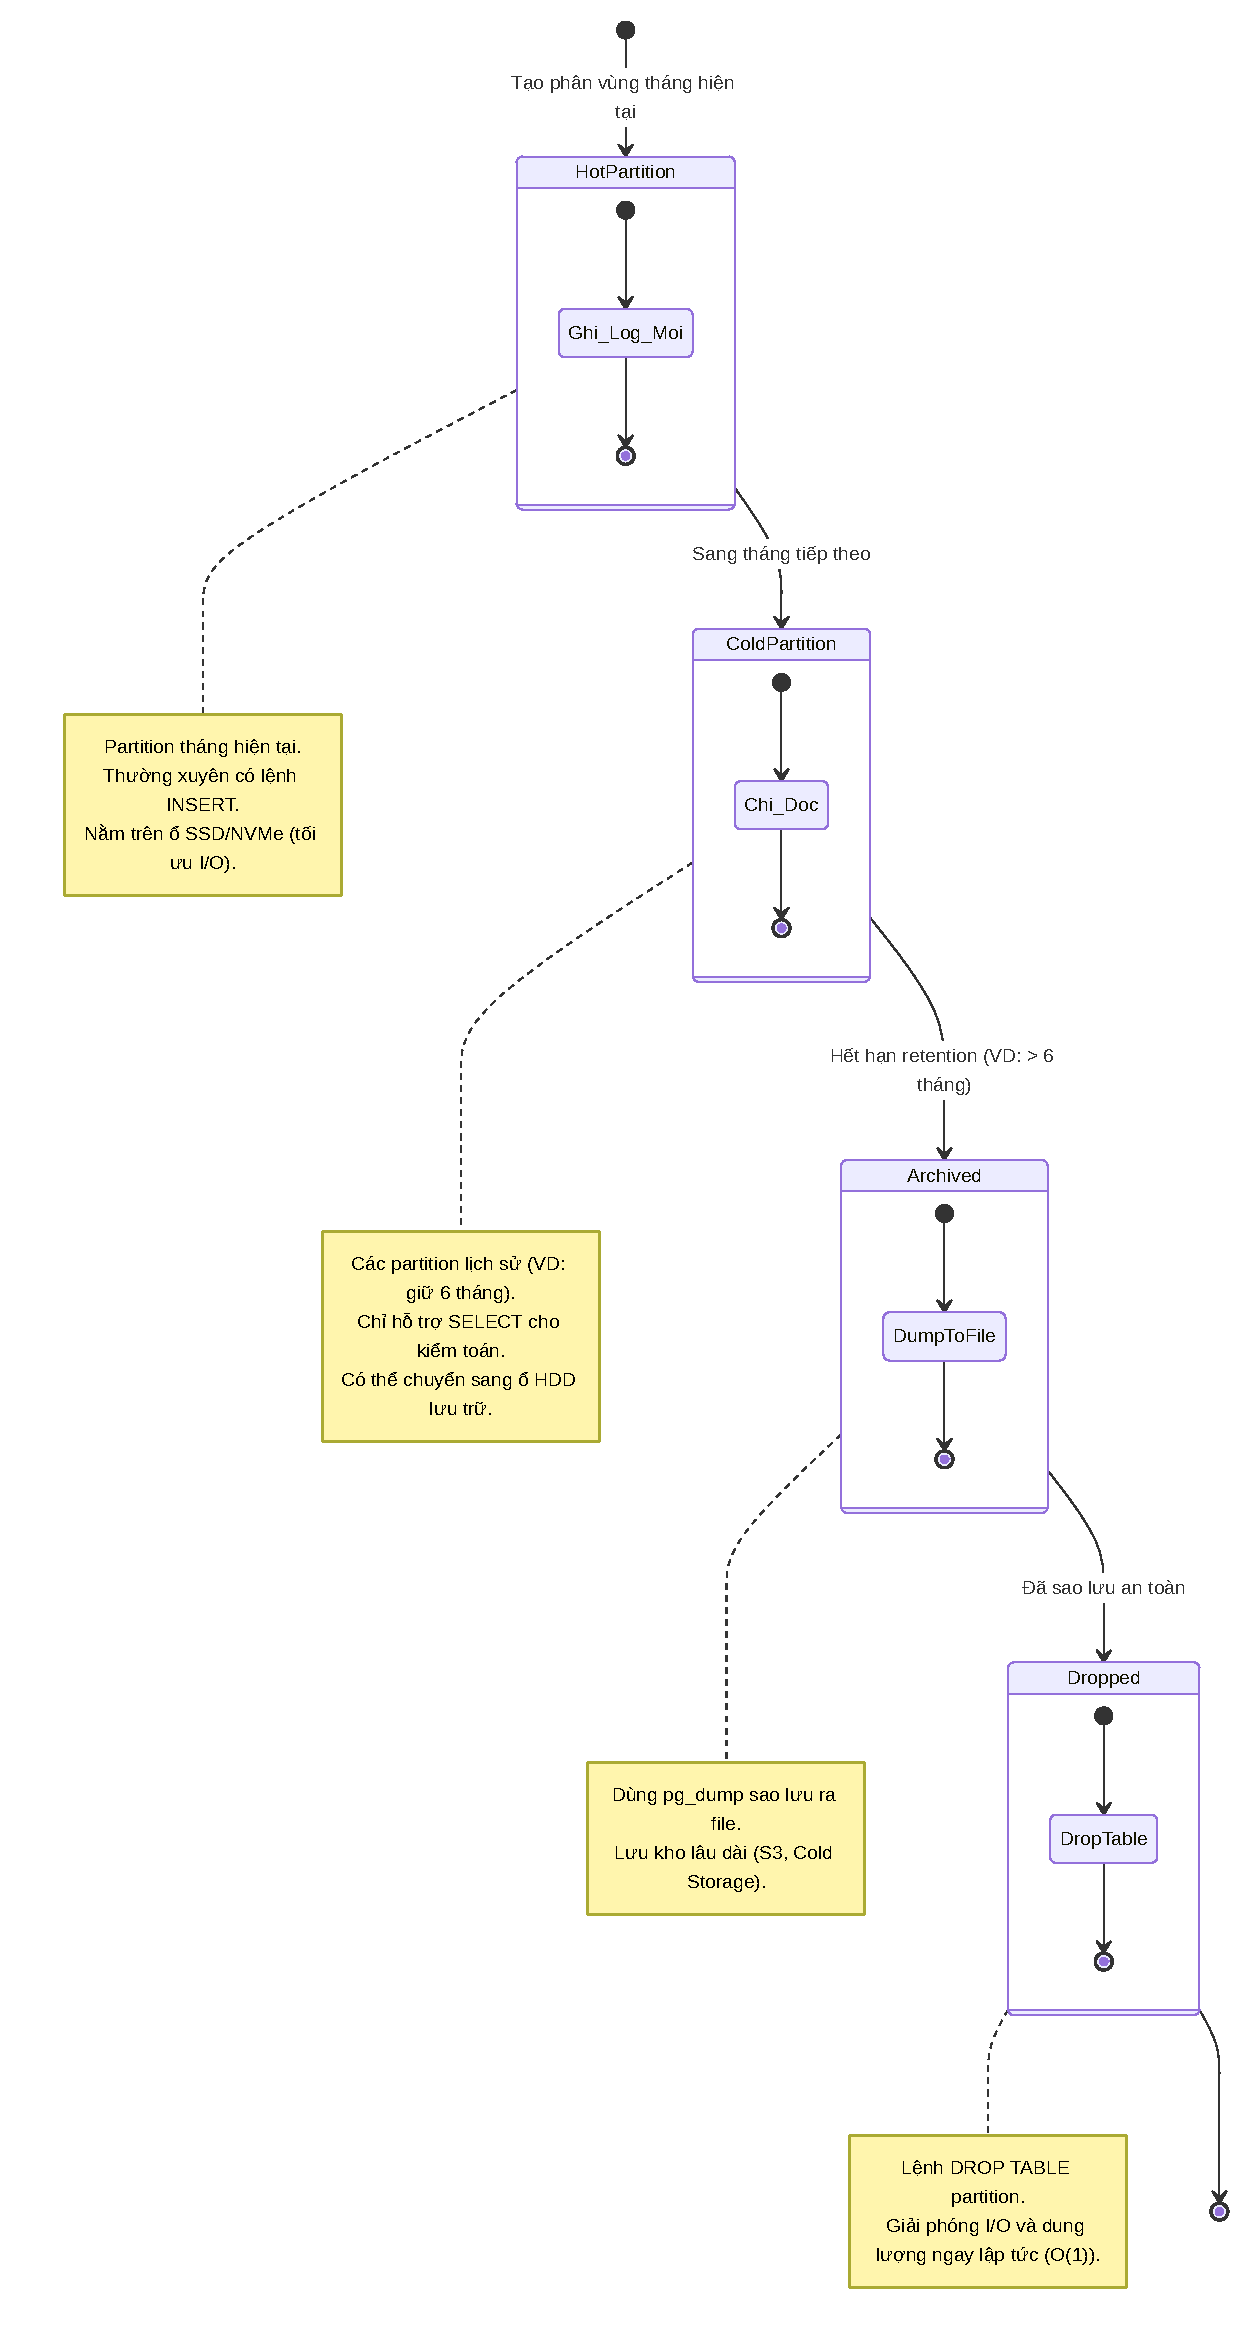
\includegraphics[width=\textwidth,height=0.85\textheight,keepaspectratio]{img/mermaid/partition_lifecycle.pdf}}
\captionof{figure}{Vòng đời phân vùng (Partition Lifecycle)}
\label{fig:partition-lifecycle}
\end{center}

\section{Cơ chế truy vấn/trích xuất log}

\textbf{Truy vấn theo bảng và thời gian:}
\begin{center}
\captionof{listing}{Truy vấn audit theo thời gian}
\label{lst:query-time}
\begin{Verbatim}[frame=single, fontsize=\footnotesize, numbers=left, numbersep=5pt, breaklines]
SELECT operation, user_name, old_data->>'status' AS old_status,
       new_data->>'status' AS new_status, changed_at
FROM audit_logs
WHERE table_name = 'public.orders'
  AND changed_at >= '2026-03-01' AND changed_at < '2026-04-01'
ORDER BY changed_at DESC LIMIT 50;
\end{Verbatim}
\end{center}

\textbf{Truy vấn sâu vào JSONB (GIN index):}
\begin{center}
\captionof{listing}{Truy vấn JSONB với toán tử containment}
\label{lst:query-jsonb}
\begin{Verbatim}[frame=single, fontsize=\footnotesize, numbers=left, numbersep=5pt, breaklines]
-- All orders shifted to PAID status
SELECT id, user_name, old_data->>'status' AS old_status, changed_at
FROM audit_logs
WHERE table_name = 'public.orders'
  AND new_data @> '{"status": "PAID"}';
-- Uses idx_audit_new_data_gin
\end{Verbatim}
\end{center}

\section{DDL Audit via Event Trigger}

Ngoài DML audit, hệ thống bổ sung \textbf{DDL audit} để ghi nhận mọi thay đổi schema (CREATE/ALTER/DROP) qua Event Trigger.

\begin{center}
\captionof{listing}{Hàm audit DDL với Event Trigger}
\label{lst:ddl-audit}
\begin{Verbatim}[frame=single, fontsize=\footnotesize, numbers=left, numbersep=5pt, breaklines]
CREATE OR REPLACE FUNCTION func_audit_ddl()
RETURNS event_trigger LANGUAGE plpgsql SECURITY DEFINER AS $$
DECLARE cmd record;
BEGIN
    FOR cmd IN SELECT * FROM pg_event_trigger_ddl_commands() LOOP
        INSERT INTO public.audit_ddl_logs
            (command_tag, object_type, object_name, command_sql, user_name)
        VALUES (
            TG_TAG,
            cmd.object_type,
            cmd.object_identity,
            cmd.command_tag || ' ' || COALESCE(cmd.object_identity, ''),
            session_user
        );
    END LOOP;
END;
$$;

CREATE EVENT TRIGGER audit_ddl_trigger
    ON ddl_command_end
    EXECUTE FUNCTION func_audit_ddl();
\end{Verbatim}
\end{center}

\textbf{Lưu ý:} Event \texttt{ddl\_command\_end} không trả về kết quả cho DROP commands --- vì khi event kích hoạt, đối tượng đã bị xóa khỏi catalog. Để bắt DROP, cần thêm event trigger riêng.

\section{Phân quyền và mô hình SECURITY DEFINER}

Hệ thống định nghĩa ba vai trò:

\begin{center}
\centering
\captionof{table}{Mô hình phân quyền ba lớp}
\label{tab:rbac}
\begin{tabularx}{\textwidth}{>{\raggedright\arraybackslash}p{3cm}>{\raggedright\arraybackslash}X>{\raggedright\arraybackslash}X}
\toprule
\textbf{Vai trò} & \textbf{Quyền trên bảng nghiệp vụ} & \textbf{Quyền trên audit\_logs} \\
\midrule
\texttt{app\_user} & SELECT, INSERT, UPDATE, DELETE & Không có \\
\texttt{auditor} & Không có & SELECT \\
\texttt{db\_admin} & ALL & ALL (owner) \\
\bottomrule
\end{tabularx}
\end{center}

\begin{sloppypar}\textbf{Hardening:} \texttt{SET search\_path = public, pg\_temp} được gắn vào mọi SECURITY DEFINER function để chống schema hijack attack.\end{sloppypar}

\section{Immutability (Append-only/WORM) cho bảng audit}
\label{sec:immutability}

\textbf{Mục tiêu:} Biến \texttt{audit\_logs} thành bảng Write-Once-Read-Many (WORM) --- một khi row được ghi, không ai --- kể cả \texttt{db\_admin} --- có thể sửa hay xóa nó.

\begin{sloppypar}\textbf{Cơ chế:} Trigger \texttt{BEFORE UPDATE OR DELETE} trên \texttt{audit\_logs} gọi hàm \texttt{func\_prevent\_\allowbreak{}audit\_change()}. Điểm then chốt là sử dụng \texttt{dblink} để ghi alert trong \textbf{autonomous transaction} độc lập --- alert được commit ngay cả khi RAISE EXCEPTION rollback transaction cha:\end{sloppypar}

\begin{center}
\captionof{listing}{Hàm WORM: chặn sửa/xóa và ghi alert qua dblink autonomous transaction}
\label{lst:worm-prevent}
\begin{Verbatim}[frame=single, fontsize=\footnotesize, numbers=left, numbersep=5pt, breaklines]
CREATE OR REPLACE FUNCTION func_prevent_audit_change()
RETURNS TRIGGER AS $$
DECLARE
    v_details JSONB;
    v_sql     TEXT;
BEGIN
    v_details := jsonb_build_object('op', TG_OP, 'schema', TG_TABLE_SCHEMA);
    IF (TG_OP = 'UPDATE') THEN
        v_details := v_details || jsonb_build_object(
            'old', to_jsonb(OLD), 'new', to_jsonb(NEW));
    ELSIF (TG_OP = 'DELETE') THEN
        v_details := v_details || jsonb_build_object('old', to_jsonb(OLD));
    END IF;

    -- Ghi alert trong transaction DOC LAP qua dblink
    -- Alert nay duoc commit ngay ca khi RAISE EXCEPTION rollback transaction cha
    v_sql := format(
        'INSERT INTO security_alerts(action,table_name,user_name,details)
         VALUES (%L,%L,%L,%L)',
        'AUDIT_TAMPER_ATTEMPT', TG_TABLE_NAME, session_user, v_details::text
    );
    PERFORM dblink_exec(
        'dbname=audit_poc host=localhost user=db_admin password=db_admin_pass',
        v_sql);

    RAISE EXCEPTION 'Audit log is immutable -- % on % denied (user: %)',
        TG_OP, TG_TABLE_NAME, session_user;
END;
$$ LANGUAGE plpgsql SECURITY DEFINER SET search_path = public, pg_temp;

CREATE TRIGGER trg_protect_audit
BEFORE UPDATE OR DELETE ON audit_logs
FOR EACH ROW EXECUTE FUNCTION func_prevent_audit_change();
\end{Verbatim}
\end{center}

\begin{center}
\centering
\makebox[\textwidth][c]{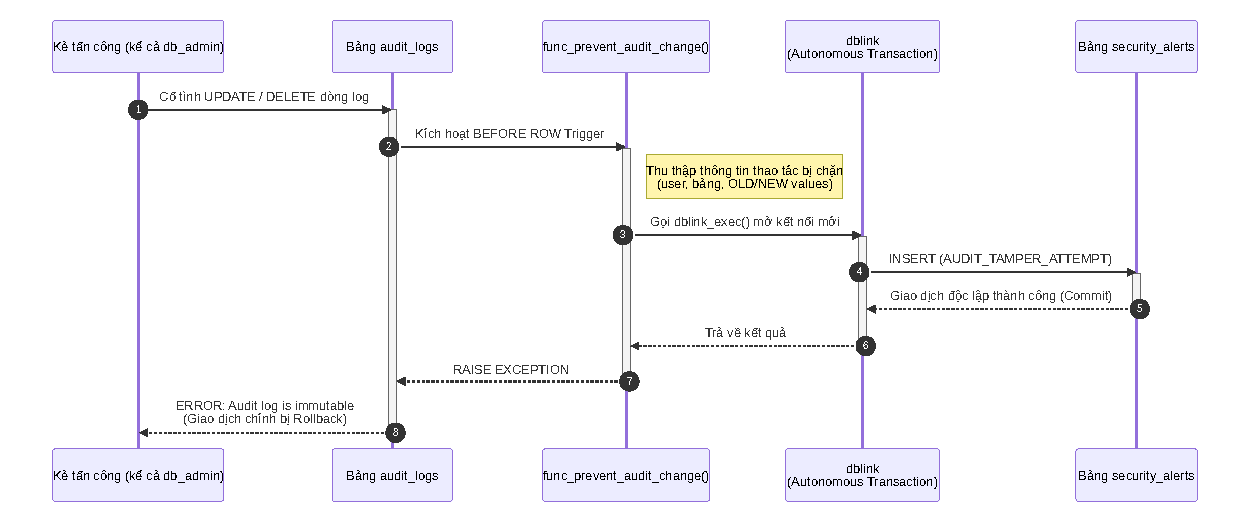
\includegraphics[width=\textwidth,height=0.85\textheight,keepaspectratio]{img/mermaid/seq_worm_dblink.pdf}}
\captionof{figure}{Sơ đồ tuần tự: Cơ chế WORM và dblink autonomous transaction}
\label{fig:seq-worm-dblink}
\end{center}

\section{Tamper-evident logging (chuỗi băm SHA-256)}

Immutability (§\ref{sec:immutability}) ngăn can thiệp qua SQL interface. Tuy nhiên, kẻ tấn công có quyền filesystem có thể sửa trực tiếp file dữ liệu PostgreSQL. Chuỗi băm SHA-256 giải quyết kịch bản này bằng cách tạo \textbf{bằng chứng toán học} không thể làm giả.

\textbf{Nguyên lý} \cite{FIPS180-4}: Mỗi log row lưu hash của chính nó và hash của row ngay trước đó:

\begin{center}
\texttt{hash\_n = SHA256(prev\_hash\_{n-1} || table\_name|operation|user\_name|old\_data|new\_data|changed\_at)}
\end{center}

\begin{center}
\captionof{listing}{Trigger hash chain (BEFORE INSERT)}
\label{lst:hash-chain}
\begin{Verbatim}[frame=single, fontsize=\footnotesize, numbers=left, numbersep=5pt, breaklines]
-- Get prev_hash from the last row
SELECT hash INTO v_prev FROM audit_logs
WHERE table_name = NEW.table_name
ORDER BY changed_at DESC, id DESC LIMIT 1;

-- Build canonical payload (concatenate audit fields)
v_payload := COALESCE(NEW.table_name, '')   || '|' ||
             COALESCE(NEW.operation, '')    || '|' ||
             COALESCE(NEW.user_name, '')    || '|' ||
             COALESCE(NEW.old_data::text, '') || '|' ||
             COALESCE(NEW.new_data::text, '') || '|' ||
             COALESCE(NEW.changed_at::text, '');

-- Compute hash: SHA256(prev_hash || payload)
NEW.prev_hash := v_prev;
NEW.hash := digest(COALESCE(v_prev, ''::bytea) || v_payload::bytea, 'sha256');
\end{Verbatim}
\end{center}

\textbf{Quy trình kiểm tra:} Hàm \texttt{func\_verify\_hash\_chain(p\_table\ TEXT)} duyệt log theo thứ tự \texttt{(changed\_at,\ id)}, tính lại hash từng row và so sánh với \texttt{hash} đã lưu.

\section{Chiến lược tối ưu hóa truy vấn (Query Optimization)}

\textbf{Nguyên tắc 1 --- Luôn kèm điều kiện thời gian (\texttt{changed\_at}):}
\textbf{Phân tích EXPLAIN:}
\begin{center}
\captionof{listing}{Phân tích EXPLAIN --- partition pruning}
\label{lst:explain-pruning}
\begin{Verbatim}[frame=single, fontsize=\footnotesize, numbers=left, numbersep=5pt, breaklines]
EXPLAIN ANALYZE
SELECT * FROM audit_logs
WHERE table_name = 'orders'
  AND changed_at >= '2026-04-01' AND changed_at < '2026-05-01';
-- Only scans partition audit_logs_2026_04
\end{Verbatim}
\end{center}

\textbf{Nguyên tắc 2 --- Dùng toán tử containment \texttt{@>} cho GIN:}
\textbf{Truy vấn JSONB tận dụng GIN index:}
\begin{center}
\captionof{listing}{Truy vấn JSONB tận dụng GIN index}
\label{lst:query-gin}
\begin{Verbatim}[frame=single, fontsize=\footnotesize, numbers=left, numbersep=5pt, breaklines]
SELECT * FROM audit_logs
WHERE new_data @> '{"status": "PAID"}';
-- Uses idx_audit_new_data_gin
\end{Verbatim}
\end{center}

\section{Giám sát và cảnh báo (Alerting)}

\begin{sloppypar}Trigger \texttt{func\_prevent\_audit\_change()} gọi \texttt{dblink\_exec()} để INSERT vào \texttt{security\_alerts} trong transaction độc lập. Việc này đảm bảo mọi nỗ lực can thiệp đều để lại dấu vết vĩnh viễn.\end{sloppypar}

\begin{center}
\centering
\makebox[\textwidth][c]{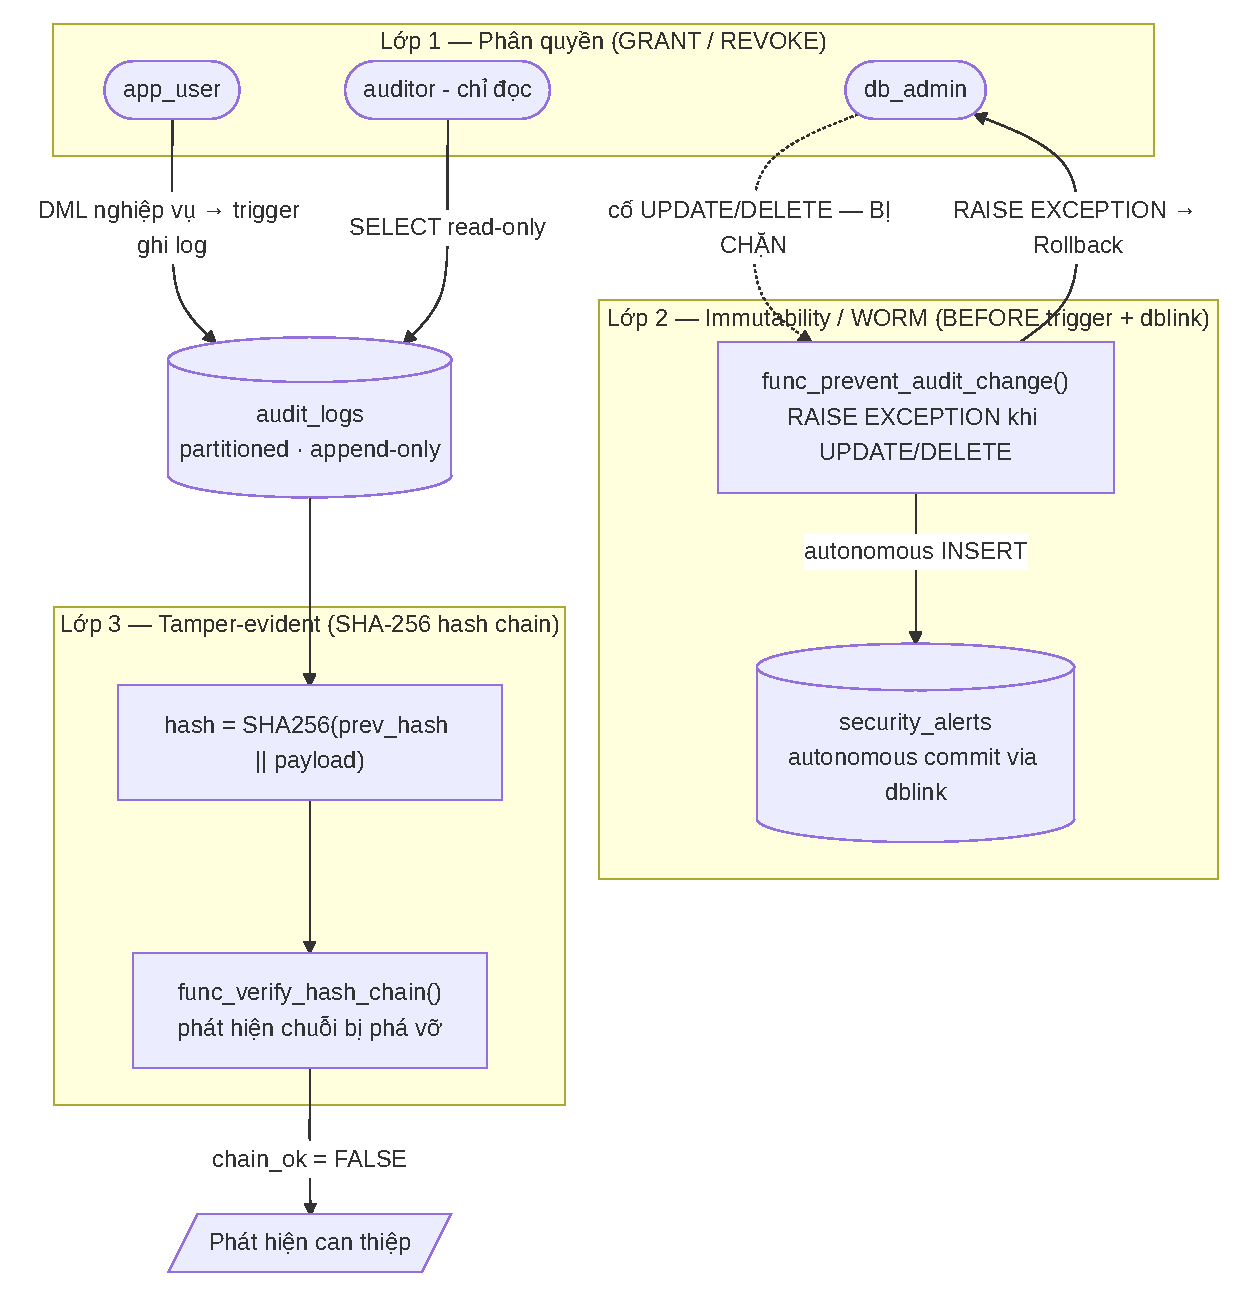
\includegraphics[width=\textwidth,height=0.85\textheight,keepaspectratio]{img/mermaid/security_3layer.pdf}}
\captionof{figure}{Kiến trúc bảo mật ba lớp}
\label{fig:security-3layer}
\end{center}

\textbf{Lớp 1 --- Phân quyền:} \texttt{app\_user} không có quyền trực tiếp trên \texttt{audit\_logs}. \textbf{Lớp 2 --- Immutability:} Trigger chặn UPDATE/DELETE, RAISE EXCEPTION đồng thời ghi alert qua dblink. \textbf{Lớp 3 --- Tamper-evident:} Hash chain SHA-256 phát hiện can thiệp ở tầng file system.
